\chapter{Results and Interpretation}
\begin{section}{Results}

The results of a background-only fit of the observed \Nb distributions are shown in Figures~\ref{fig:fit_bonly_cr} and \ref{fig:fit_bonly_sr}.
These figures separately show the $\Nleps = 1$ control and signal regions, although the fit includes all bins simultaneously.
The \Nb distributions in data are well described by the fit, and examination of the nuisance parameters shows that none of them are significantly changed by the fit.
The post-fit yields are presented in Table~\ref{tab:fit_bonly_yields}.

\begin{figure}[tbp!]
\centering
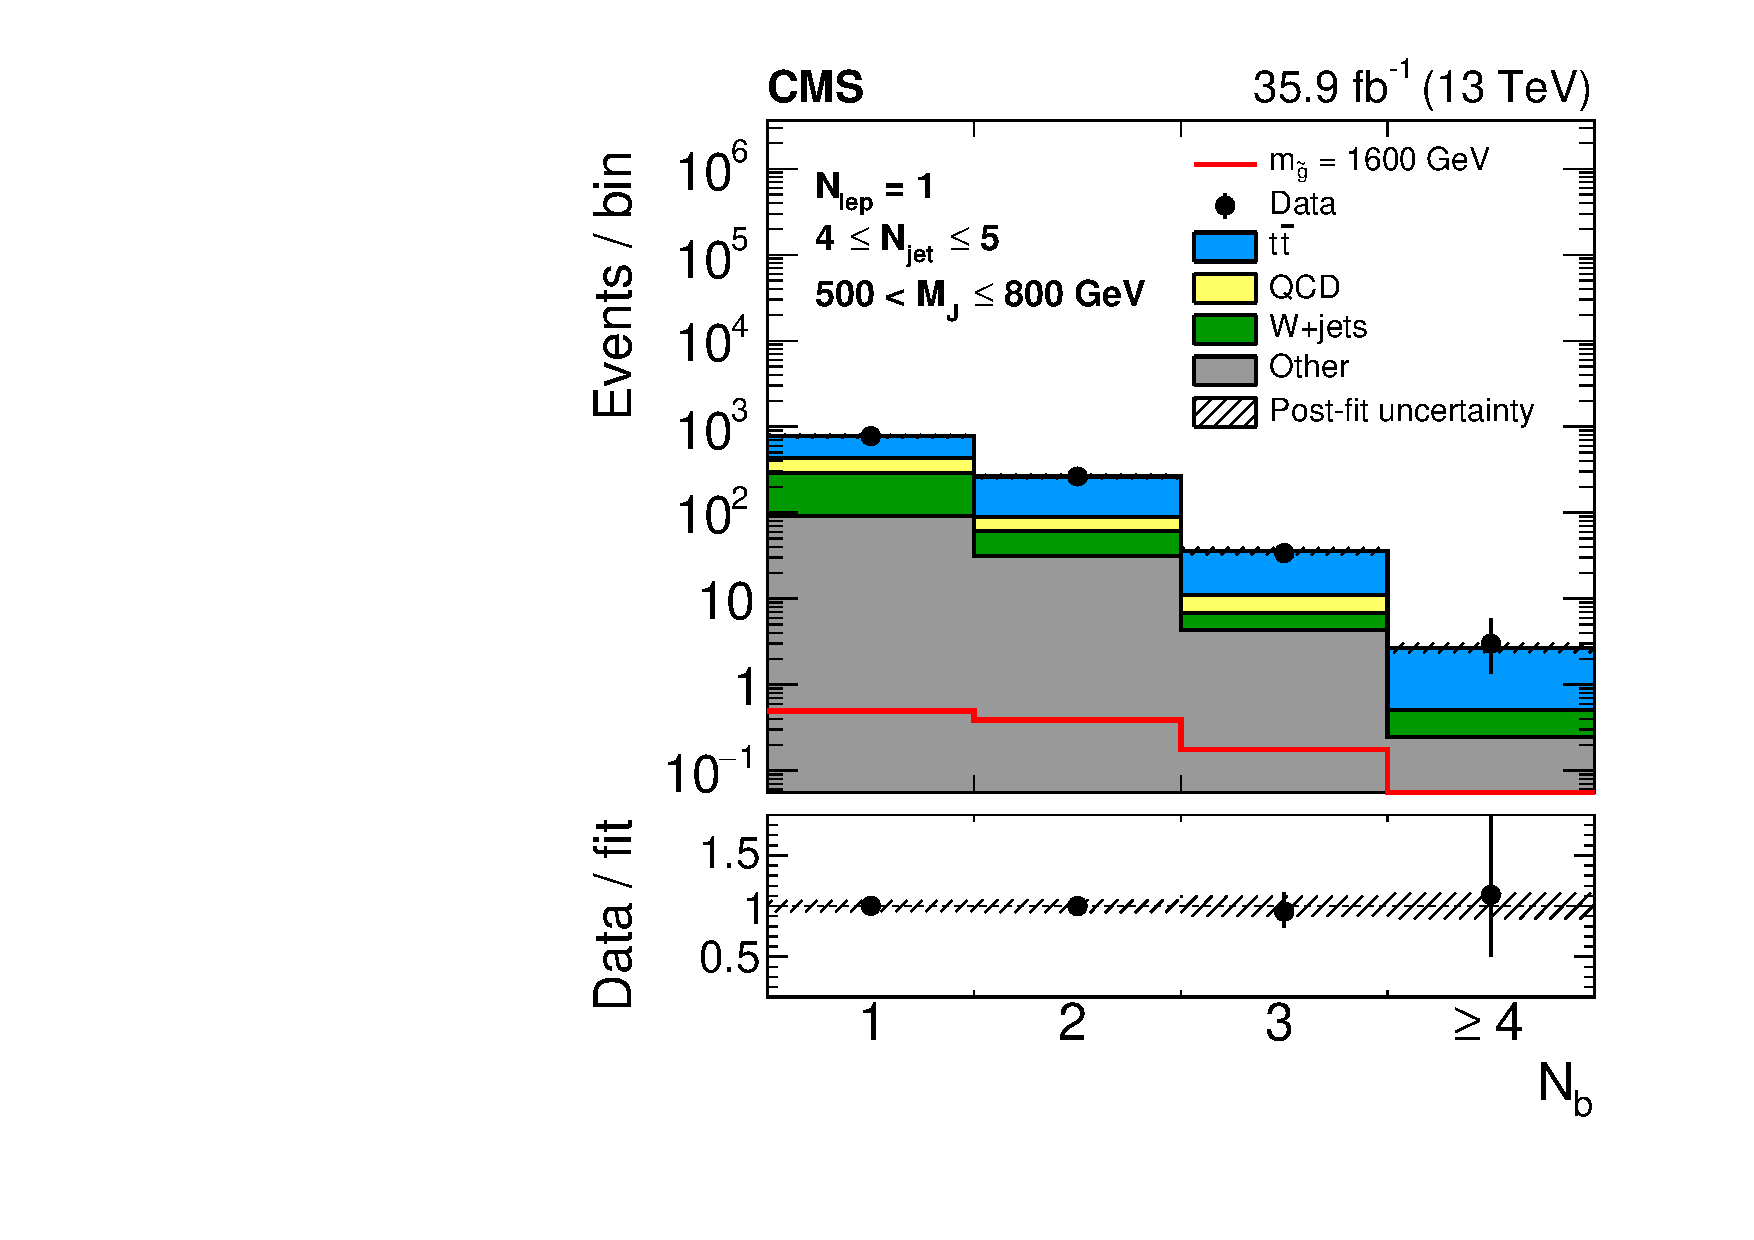
\includegraphics[angle=0,width=0.45\columnwidth]{fig/fit_nlep1_nj45_lowmj.pdf}
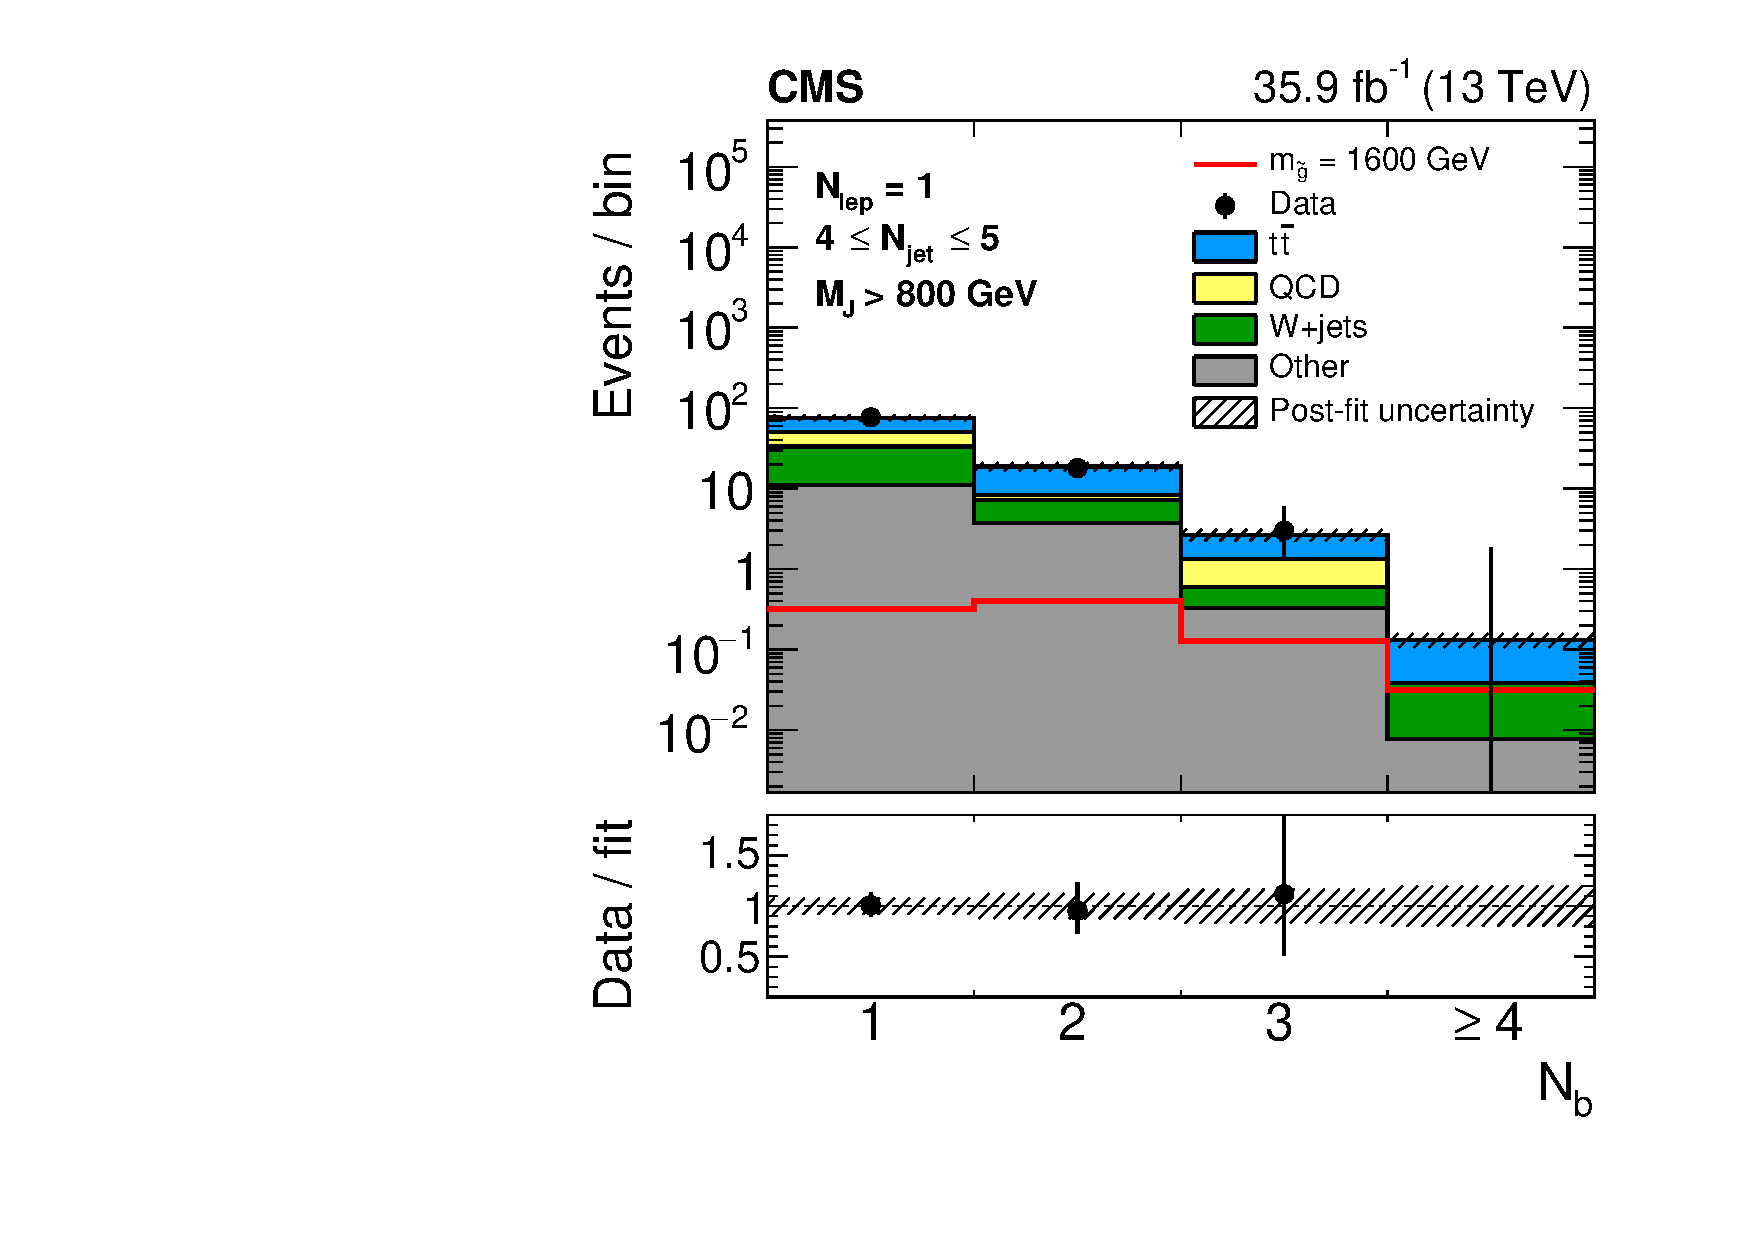
\includegraphics[angle=0,width=0.45\columnwidth]{fig/fit_nlep1_nj45_highmj.pdf}
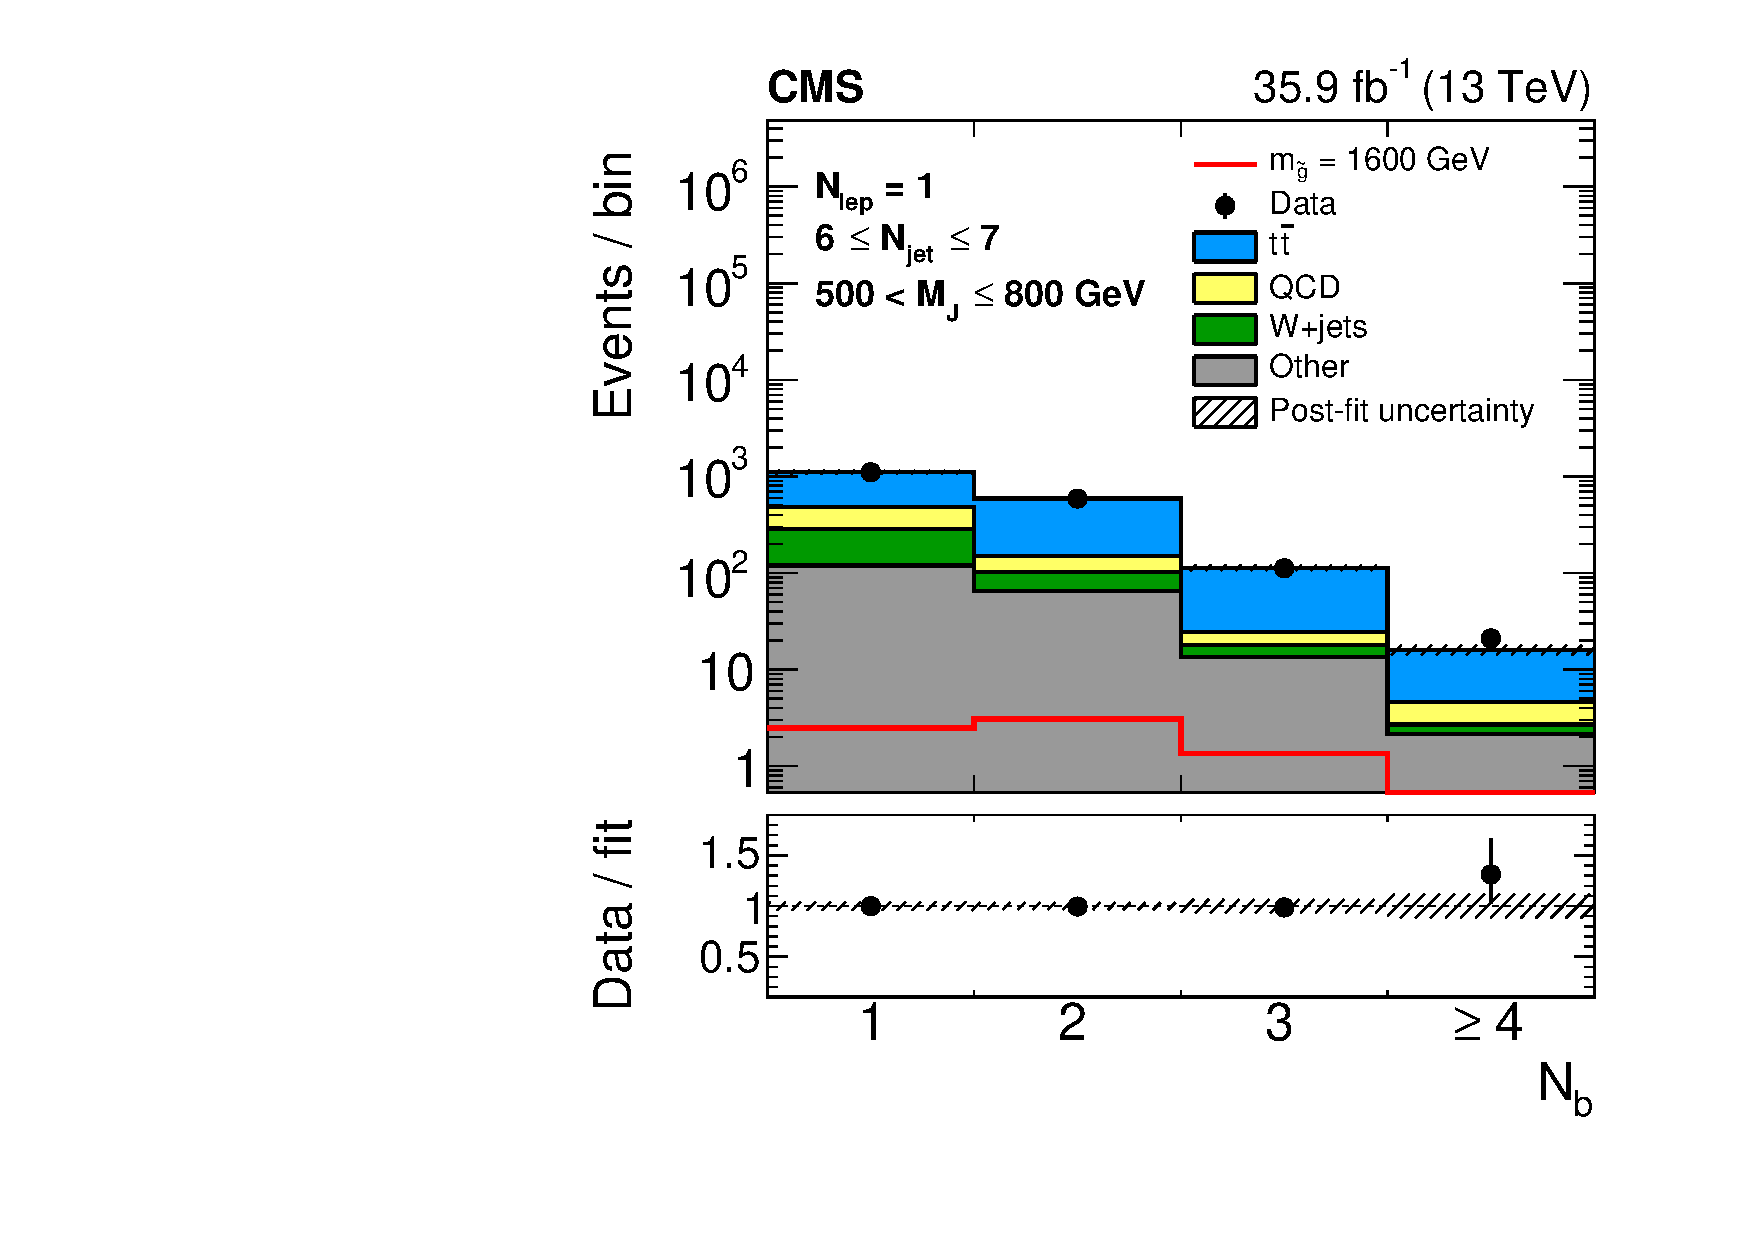
\includegraphics[angle=0,width=0.45\columnwidth]{fig/fit_nlep1_nj67_lowmj.pdf}
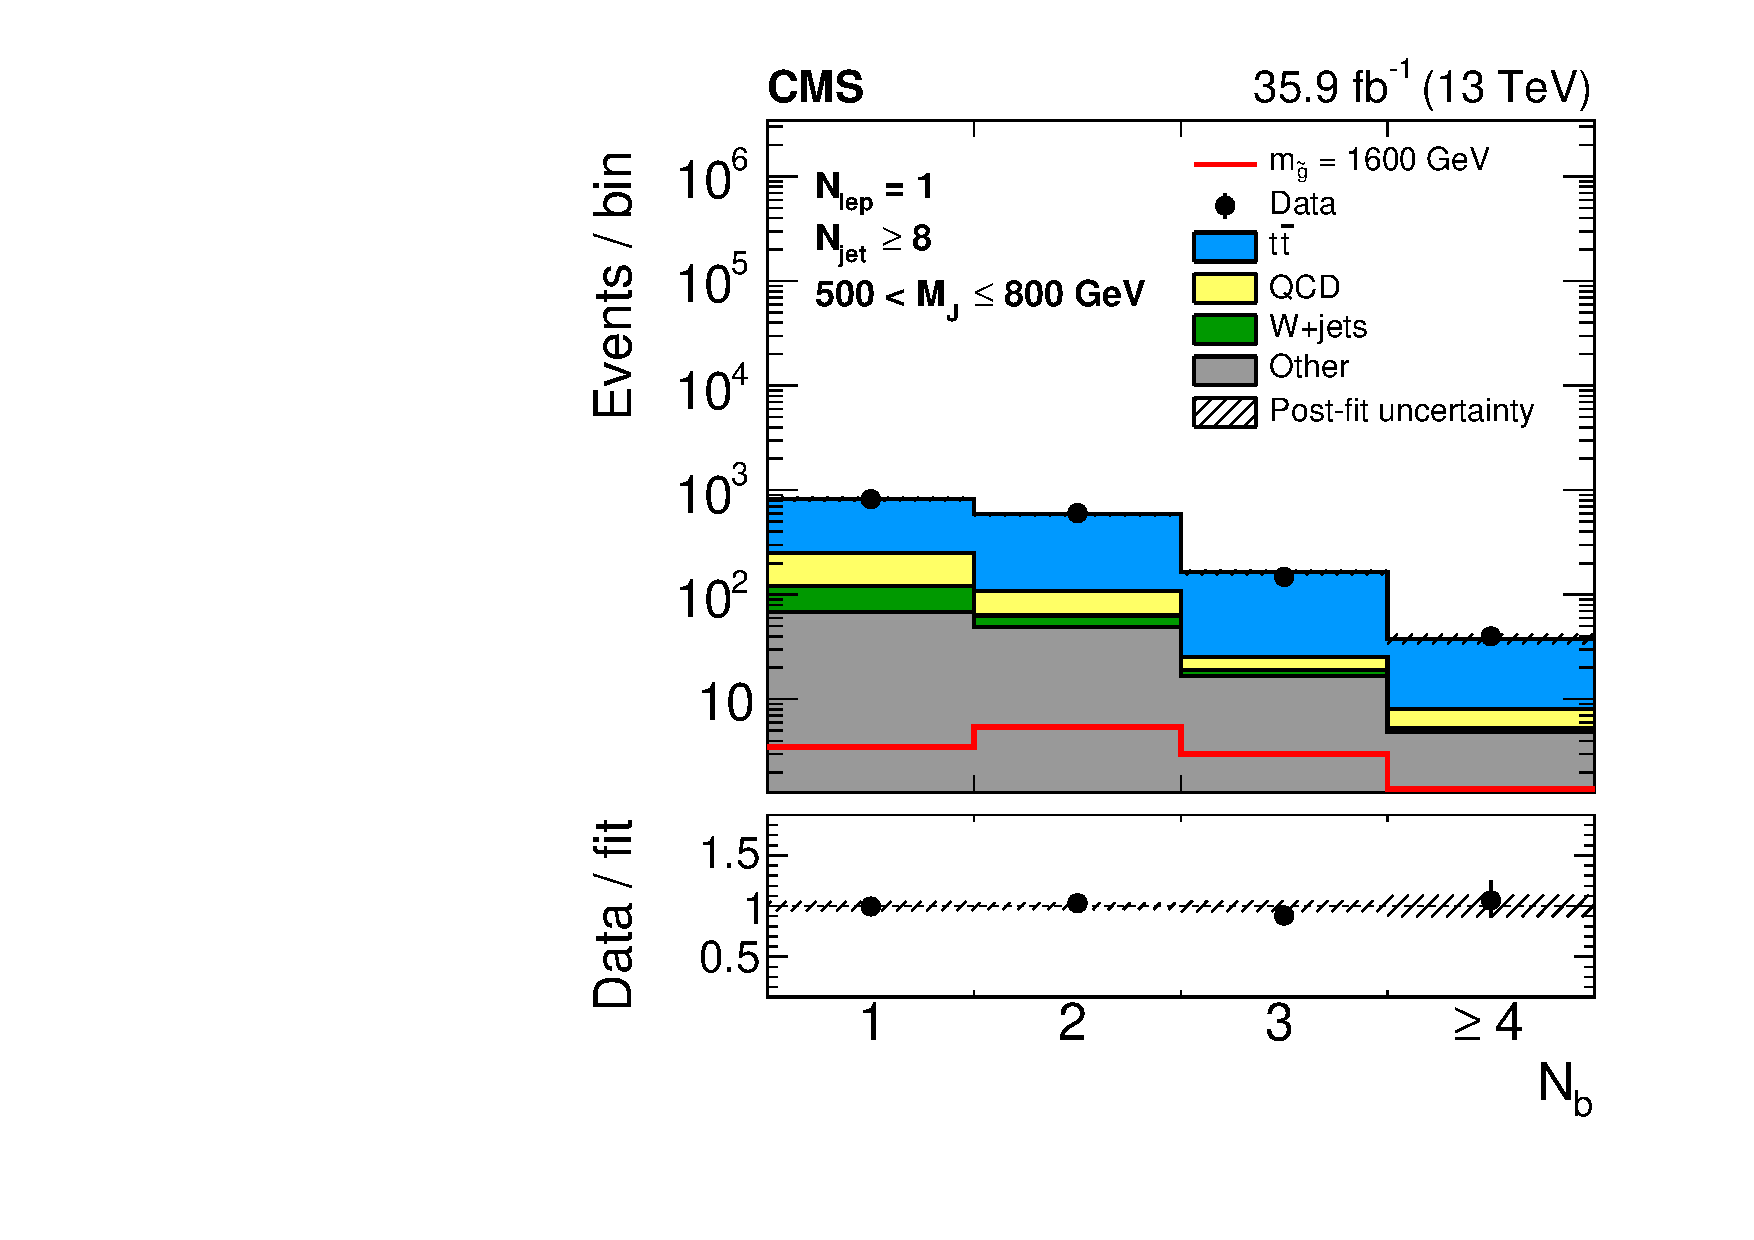
\includegraphics[angle=0,width=0.45\columnwidth]{fig/fit_nlep1_nj8_lowmj.pdf}
\caption{Data and the background-only post-fit \Nb distribution for bins with low expected signal contribution: $4 \leq \Njets \leq 5$, $500 < \MJ \leq 800~\GeV$ (upper-left), $4 \leq \Njets \leq 5$, $\MJ > 800~\GeV$ (upper-right), $6 \leq \Njets \leq 7$, $500 < \MJ \leq 800~\GeV$ (lower-left), and $\Njets \geq 8$, $500 < \MJ \leq 800~\GeV$ (lower-right).
The expected signal distribution is also shown for a gluino mass of 1600~\GeV.
The ratio of data to post-fit yields is shown in the lower panel.
The post-fit uncertainty is depicted as a hatched band.}
\label{fig:fit_bonly_cr}
\end{figure}

\begin{figure}[tbp!]
\centering
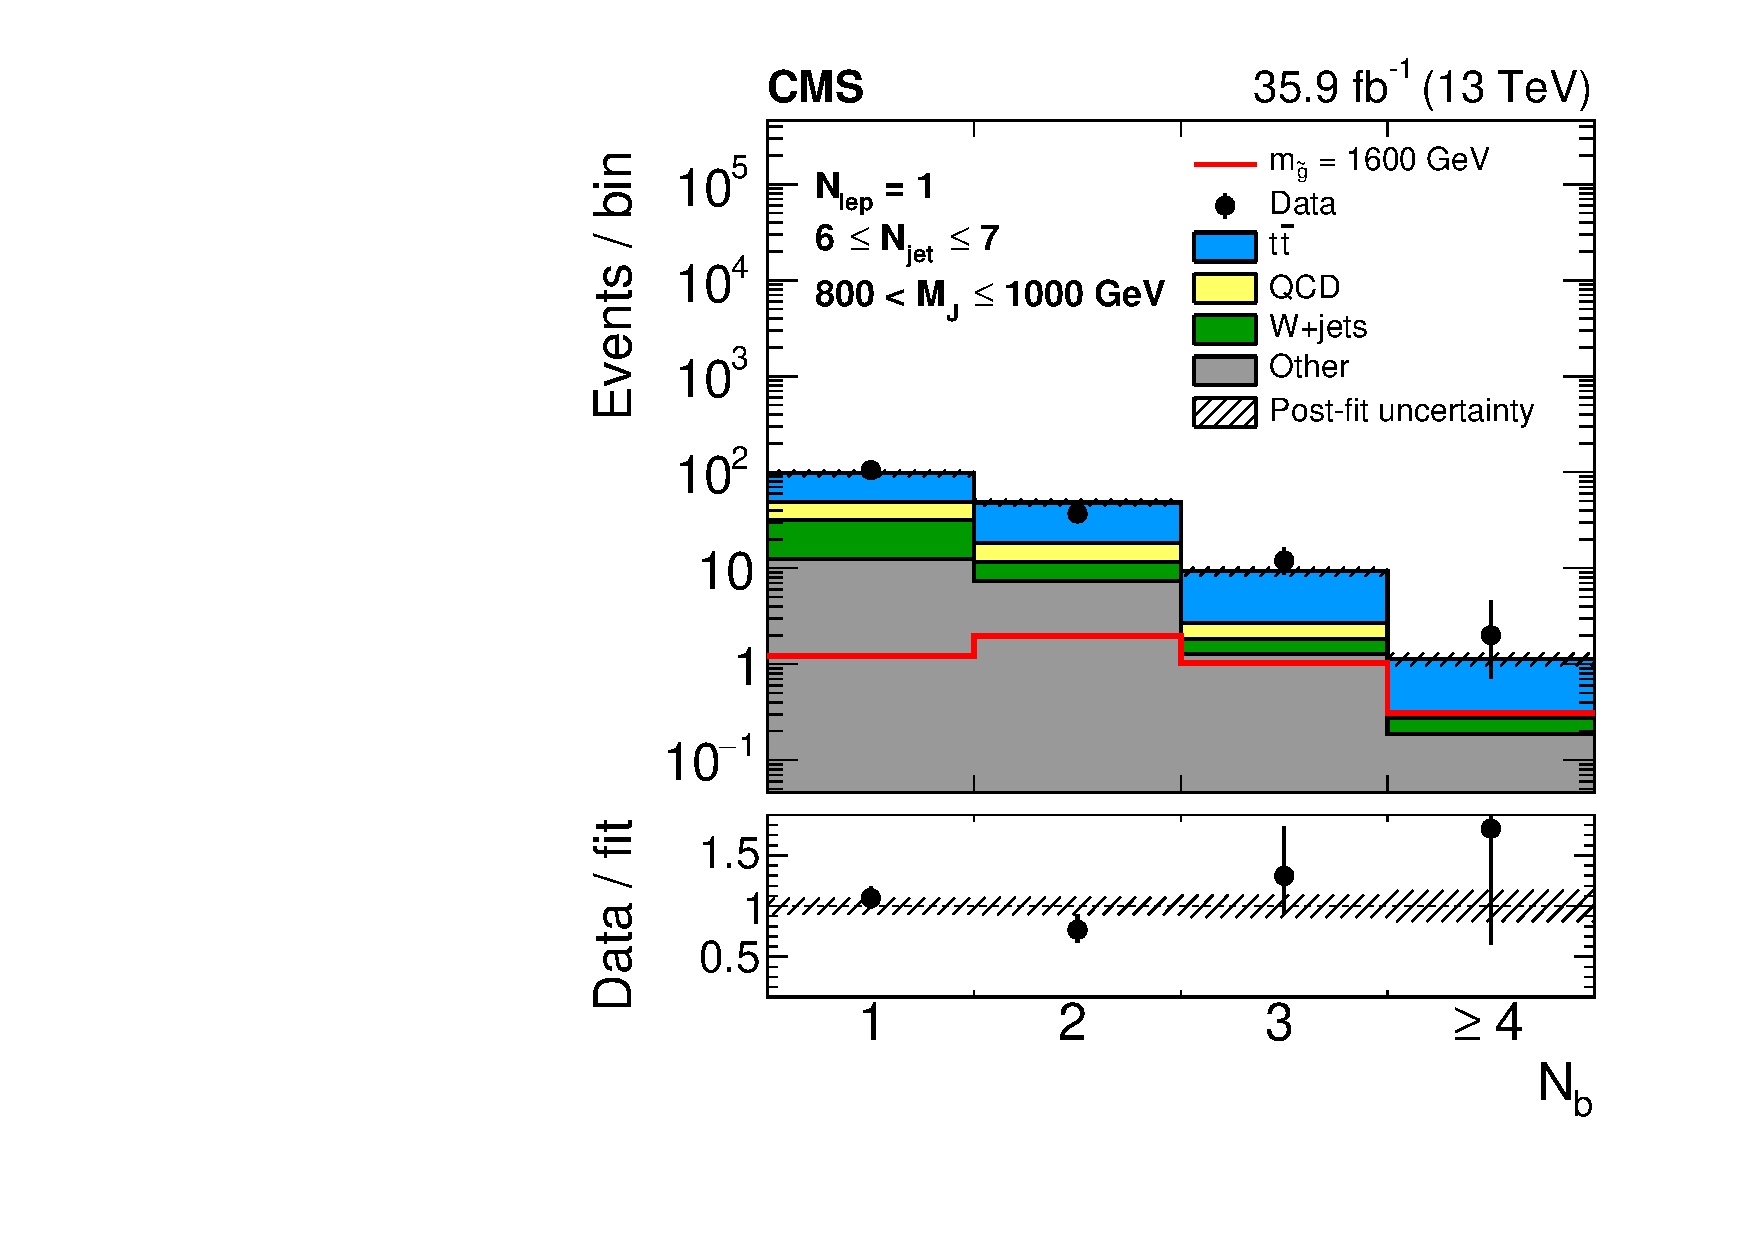
\includegraphics[angle=0,width=0.45\columnwidth]{fig/fit_nlep1_nj67_highmj.pdf}
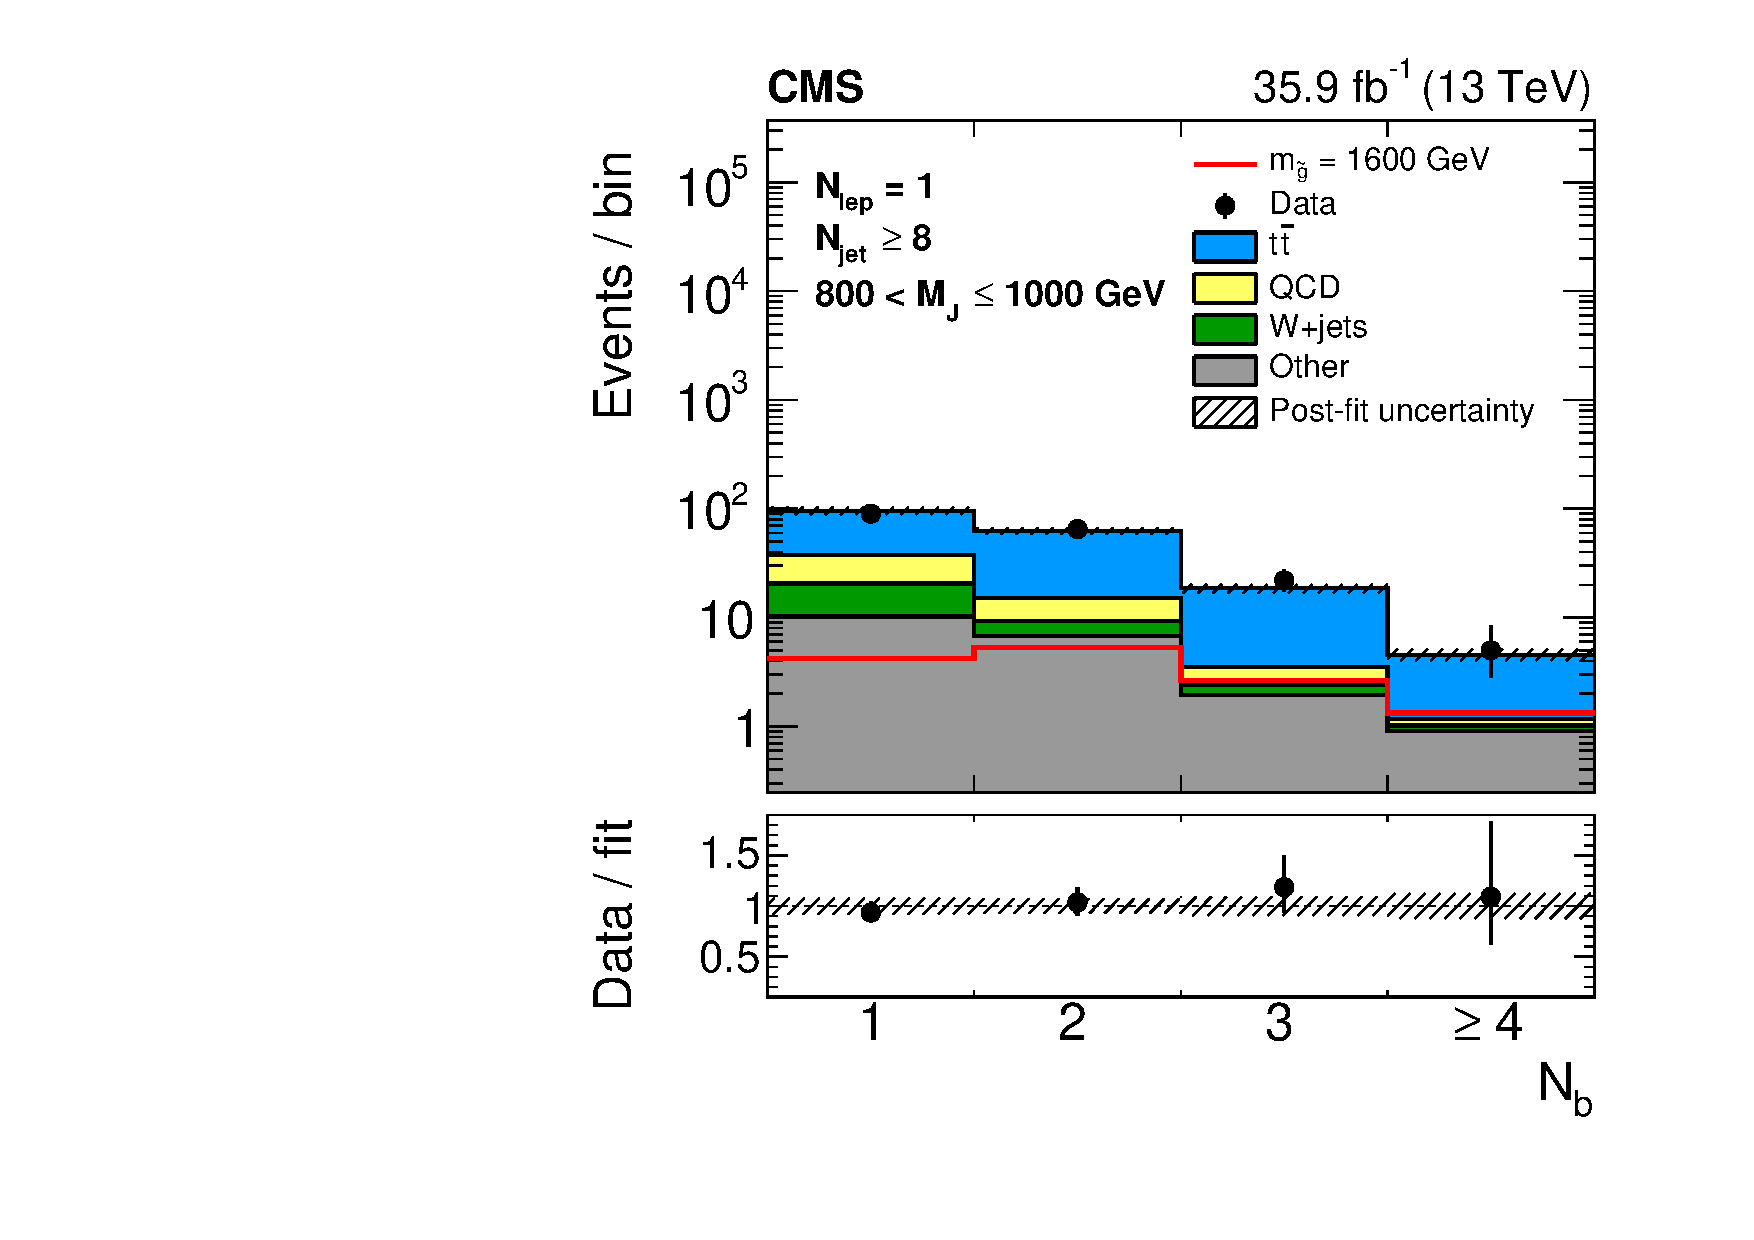
\includegraphics[angle=0,width=0.45\columnwidth]{fig/fit_nlep1_nj8_highmj.pdf}
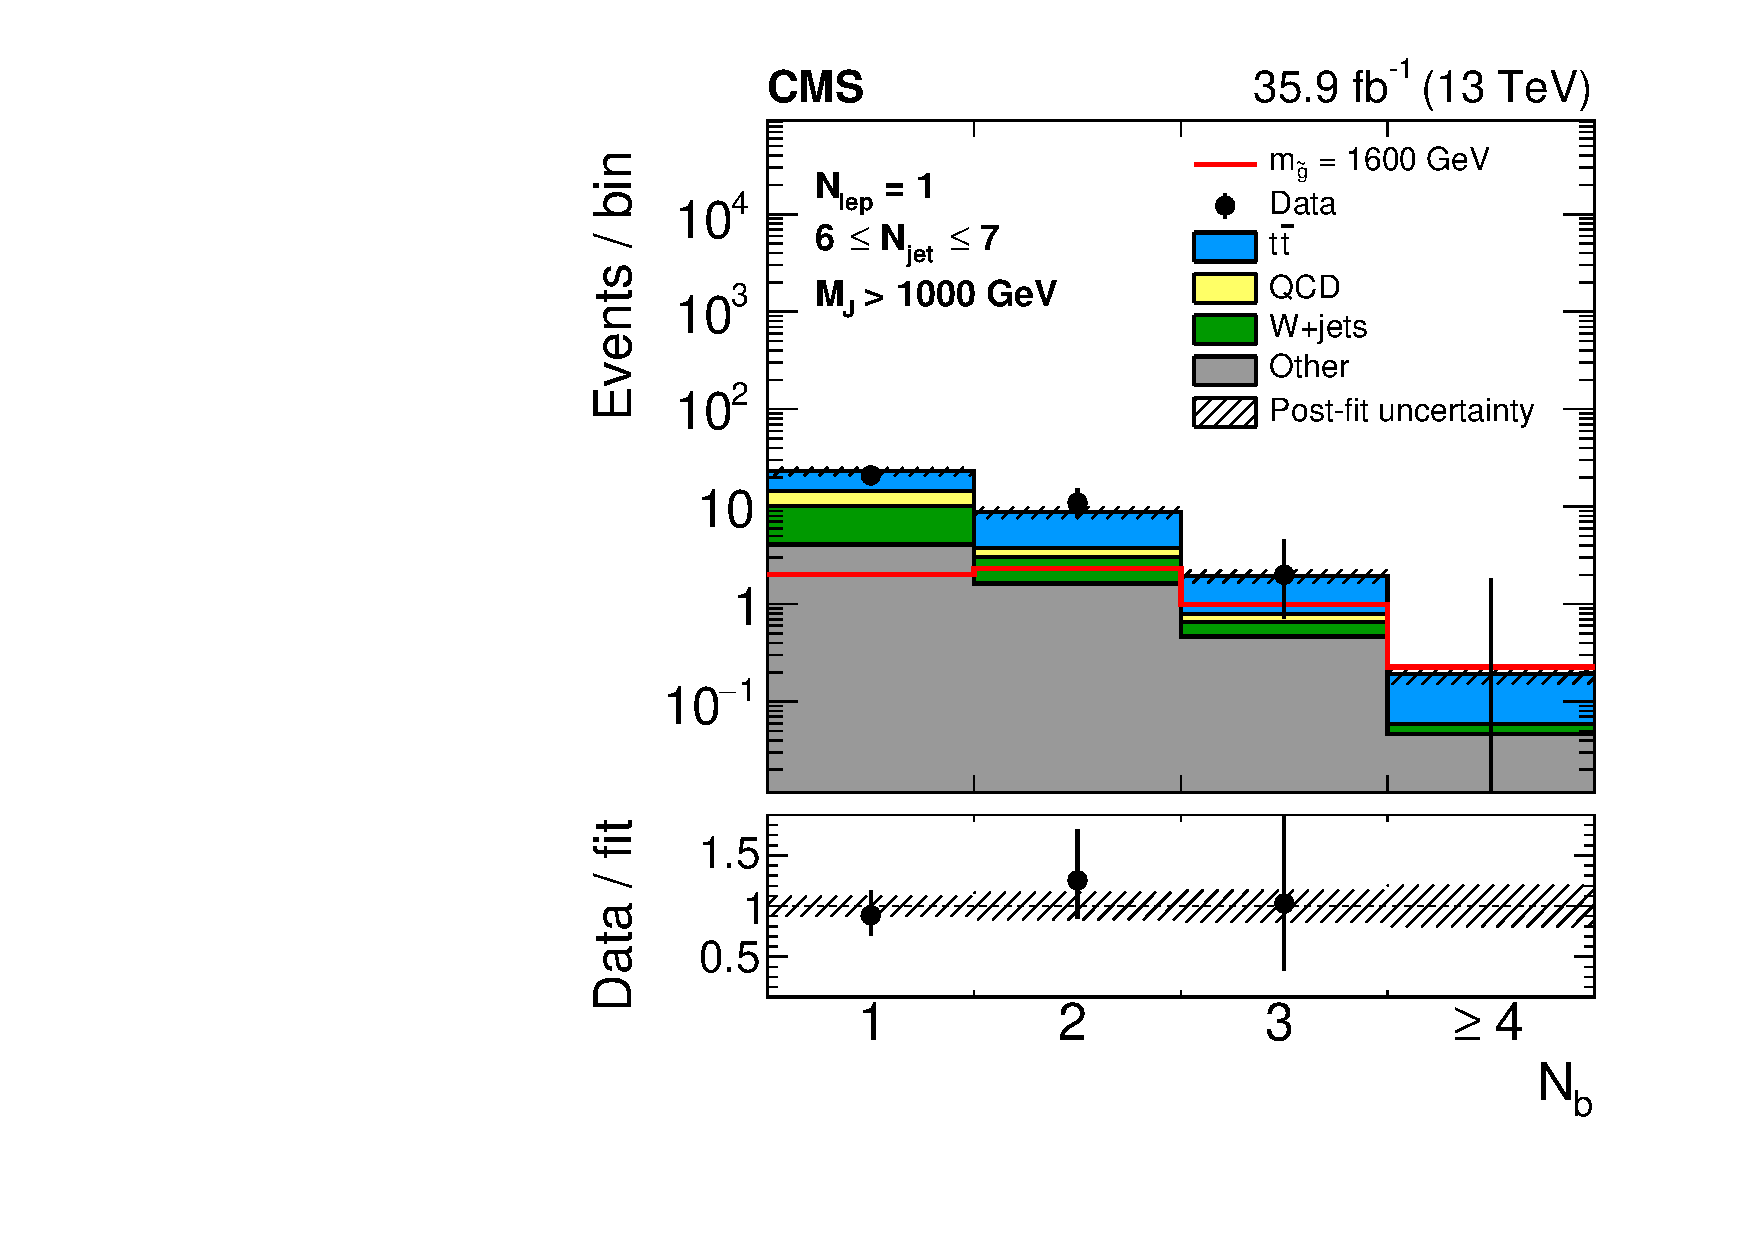
\includegraphics[angle=0,width=0.45\columnwidth]{fig/fit_nlep1_nj67_vhighmj.pdf}
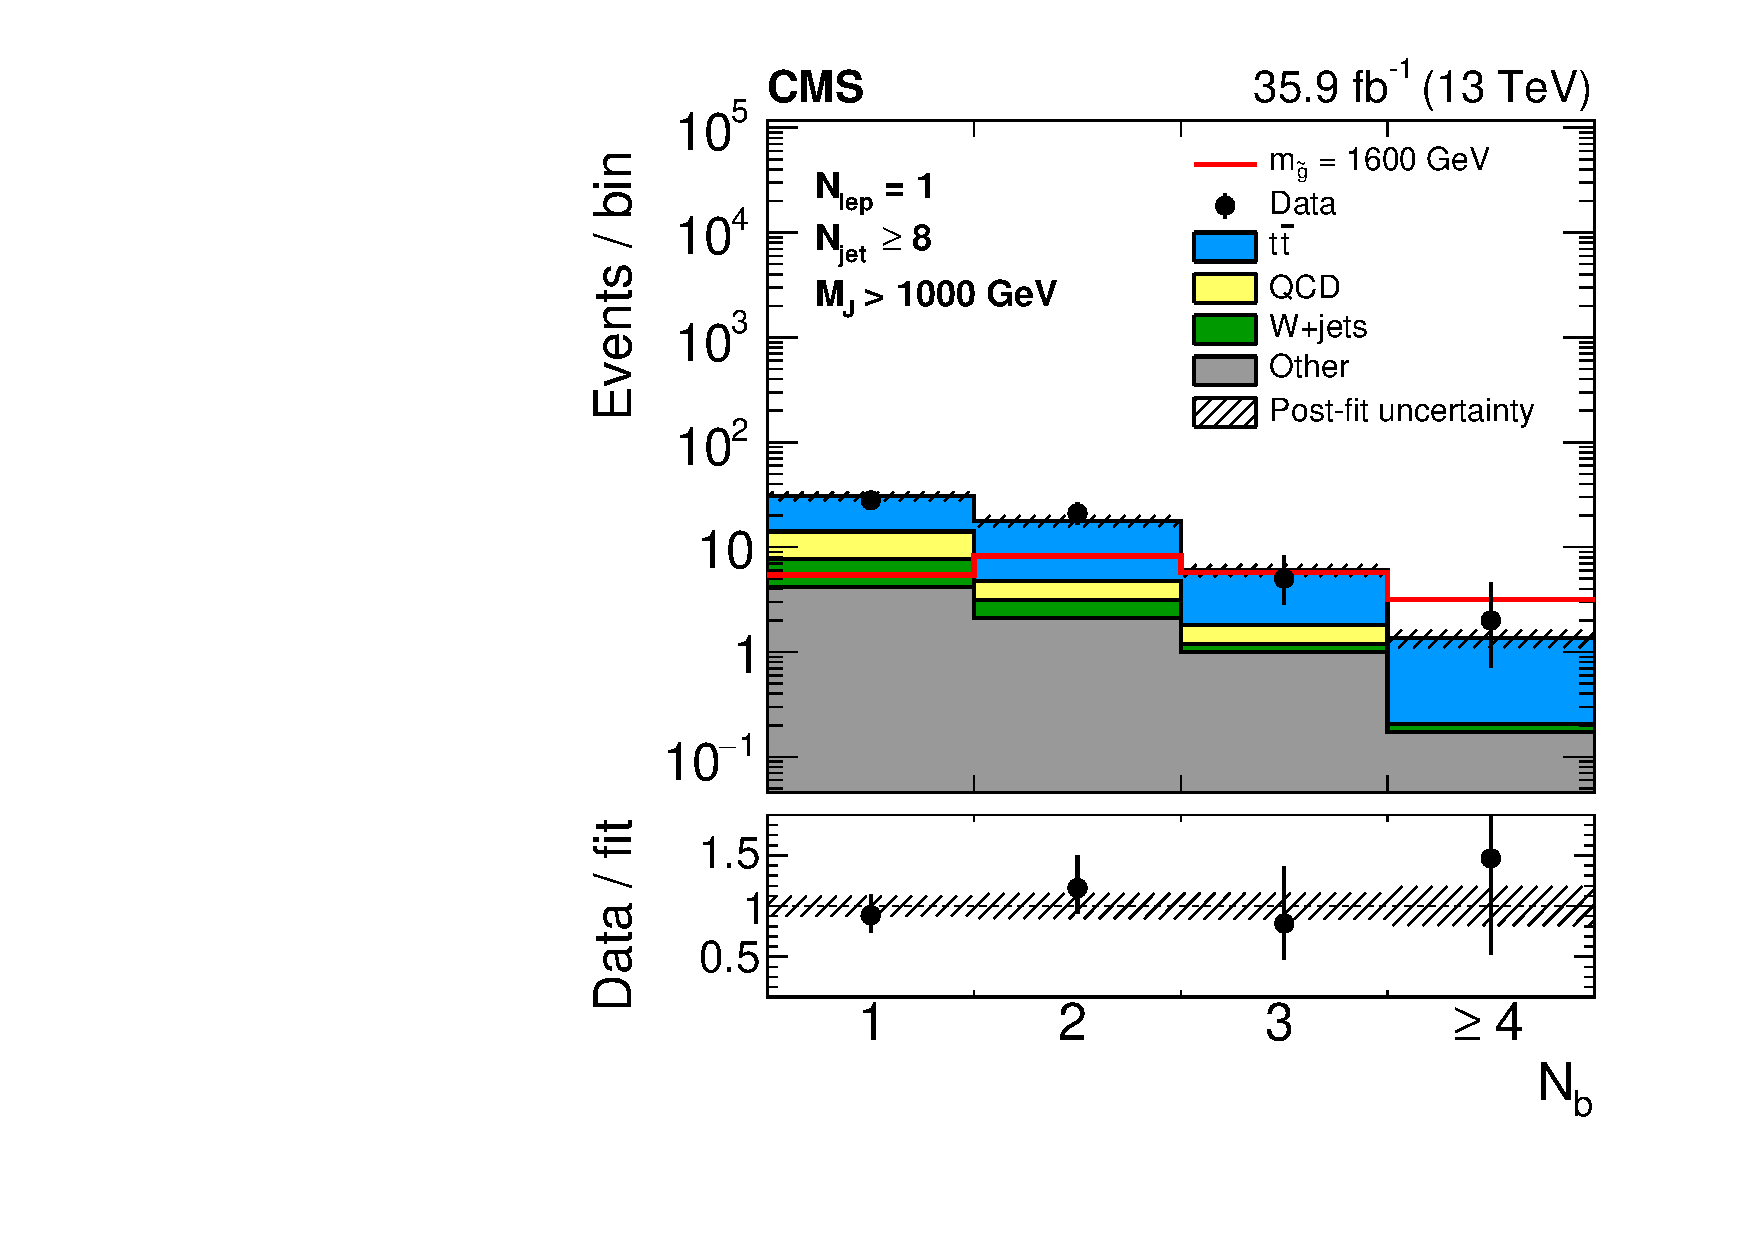
\includegraphics[angle=0,width=0.45\columnwidth]{fig/fit_nlep1_nj8_vhighmj.pdf}
\caption{Data and the background-only post-fit \Nb distribution for bins with large expected signal contribution: $6 \leq \Njets \leq 7$, $800 < \MJ \leq 1000~\GeV$ (upper-left), $\Njets \geq 8$, $800 < \MJ \leq 1000~\GeV$ (upper-right), $ 6 \leq \Njets \leq 7$, $\MJ > 1000~\GeV$ (lower-left), and $ \Njets \geq 8$, $\MJ > 1000~\GeV$ (lower-right).
The expected signal distribution is also shown for a gluino mass of 1600~\GeV.
The ratio of data to post-fit yields is shown in the lower panel.
The post-fit uncertainty is depicted as a hatched band.}
\label{fig:fit_bonly_sr}
\end{figure}

\begin{table}
\centering
\begin{tabular}[tbp!]{ l | c  c  c  c | c |  c | c  }
\hline
$\Nb$    & QCD    & \ttbar  & \Wjets & Other  & All bkg.      & Data   & Expected $\mglu = 1600~\GeV$ \\
\hline
\multicolumn{8}{c}{$4 \leq \Njets \leq 5$, $500 < \MJ \leq 800~\GeV$} \\
\hline
$1$      & $148$  & $340$   & $196$  & $91$   & $775\pm43$    & $777$  & $0.50 \pm 0.13$ \\
$2$      & $29$   & $175$   & $30$   & $31$   & $264\pm17$    & $264$  & $0.39 \pm 0.11$ \\
$3$      & $4.3$  & $24.8$  & $2.5$  & $4.4$  & $36\pm4$      & $34$   & $0.18 \pm 0.08$ \\
$\geq 4$ & $0.0$  & $2.2$   & $0.3$  & $0.2$  & $2.7\pm0.4$   & $3$    & $0.04 \pm 0.04$ \\
\hline
\multicolumn{8}{c}{$4 \leq \Njets \leq 5$, $\MJ > 800~\GeV$} \\
\hline
$1$      & $16.5$ & $26.3$  & $22.5$ & $11.0$ & $76\pm6$      & $77$   & $0.32 \pm 0.11$ \\
$2$      & $1.1$  & $10.6$  & $3.4$  & $3.8$  & $19\pm2$      & $18$   & $0.40 \pm 0.12$ \\
$3$      & $0.7$  & $1.3$   & $0.3$  & $0.3$  & $2.7\pm0.5$   & $3$    & $0.13 \pm 0.06$ \\
$\geq 4$ & $0.00$ & $0.09$  & $0.03$ & $0.01$ & $0.13\pm0.03$ & $0$    & $0.03 \pm 0.03$ \\
\hline
\multicolumn{8}{c}{$6 \leq \Njets \leq 7$, $500 < \MJ \leq 800~\GeV$} \\
\hline
$1$      & $197$  & $620$   & $169$  & $120$  & $1106\pm48$   & $1105$ &  $2.5 \pm 0.3$  \\
$2$      & $49$   & $440$   & $36$   & $66$   & $591\pm21$    & $588$  & $3.1 \pm 0.3$   \\
$3$      & $6.4$  & $89.2$  & $4.6$  & $13.4$ & $114\pm8$     & $112$  & $1.4 \pm 0.2$   \\
$\geq 4$ & $1.9$  & $11.4$  & $0.6$  & $2.1$  & $16\pm2$      & $21$   & $0.25 \pm 0.09$ \\
\hline
\multicolumn{8}{c}{$\Njets \geq 8$, $500 < \MJ \leq 800~\GeV$} \\
\hline
$1$      & $130$  & $574$   & $53$   & $68$   & $825\pm38$    & $821$  & $3.5 \pm 0.3$   \\
$2$      & $45$   & $478$   & $14$   & $49$   & $586\pm20$    & $603$  & $5.4 \pm 0.4$   \\
$3$      & $6.3$  & $138.1$ & $2.5$  & $16.7$ & $164\pm9$     & $148$  & $3.0 \pm 0.3$   \\
$\geq 4$ & $2.8$  & $29.8$  & $0.4$  & $4.8$  & $38\pm4$      & $40$   &  $1.4 \pm 0.2$  \\
\hline
\multicolumn{8}{c}{$6 \leq \Njets \leq 7$, $800 < \MJ \leq 1000~\GeV$} \\
\hline
$1$      & $17.3$ & $48.4$  & $19.2$ & $12.3$ & $97\pm8$      & $105$  & $1.2 \pm 0.2$   \\
$2$      & $6.6$  & $30.1$  & $4.3$  & $7.3$  & $48\pm4$      & $37$   & $2.0 \pm 0.3$   \\
$3$      & $0.8$  & $6.6$   & $0.5$  & $1.3$  & $9.3\pm1.0$   & $12$   & $1.0 \pm 0.2$   \\
$\geq 4$ & $0.0$  & $0.9$   & $0.1$  & $0.2$  & $1.1\pm0.2$   & $2$    & $0.31 \pm 0.09$ \\
\hline
\multicolumn{8}{c}{$\Njets \geq 8$, $800 < \MJ \leq 1000~\GeV$} \\
\hline
$1$      & $17.0$ & $58.7$  & $10.3$ & $10.2$ & $96\pm8$      & $90$   & $4.2 \pm 0.4$   \\
$2$      & $5.8$  & $47.5$  & $2.5$  & $6.8$  & $63\pm5$      & $65$   & $5.3 \pm 0.4$   \\
$3$      & $1.1$  & $15.0$  & $0.4$  & $2.0$  & $19\pm2$      & $22$   & $2.6 \pm 0.3$   \\
$\geq 4$ & $0.2$  & $3.4$   & $0.1$  & $0.9$  & $4.6\pm0.6$   & $5$    & $1.3 \pm 0.2$   \\
\hline
\multicolumn{8}{c}{$6 \leq \Njets \leq 7$, $\MJ > 1000~\GeV$} \\
\hline
$1$      & $4.4$  & $8.7$   & $6.0$  & $4.1$  & $23\pm2$      & $21$   & $2.0 \pm 0.3$   \\
$2$      & $0.7$  & $5.0$   & $1.4$  & $1.6$  & $8.8\pm1.2$   & $11$   & $2.3 \pm 0.3$   \\
$3$      & $0.1$  & $1.2$   & $0.2$  & $0.5$  & $1.9\pm0.3$   & $2$    & $1.0 \pm 0.2$   \\
$\geq 4$ & $0.00$ & $0.13$  & $0.01$ & $0.05$ & $0.19\pm0.04$ & $0$    & $0.23 \pm 0.08$ \\
\hline
\multicolumn{8}{c}{$\Njets \geq 8$, $\MJ > 1000~\GeV$} \\
\hline
$1$      & $6.4$  & $16.7$  & $3.5$  & $4.1$  & $31\pm3$      & $28$   & $5.4 \pm 0.4$   \\
$2$      & $1.6$  & $13.1$  & $1.1$  & $2.1$  & $18\pm2$      & $21$   & $8.2 \pm 0.5$   \\
$3$      & $0.6$  & $4.2$   & $0.2$  & $1.0$  & $6.0\pm0.8$   & $5$    & $5.7 \pm 0.4$   \\
$\geq 4$ & $0.0$  & $1.2$   & $0.0$  & $0.2$  & $1.4\pm0.3$   & $2$    & $3.2 \pm 0.3$   \\
\hline
\end{tabular}
\caption{Post-fit yields of the background-only fit, observed data, and expected yields for $\mglu = 1600~\GeV$.}
\label{tab:fit_bonly_yields}
\end{table}

A signal-plus-background fit is performed for gluino masses ranging from 1000 to 2000~\GeV.
For all masses, the post-fit \Nb distribution describes the data well, and the fit extracts at most a small and insignificant signal contribution.
For example, with a 1600~\GeV gluino, the extracted signal yield relative to the model prediction is $r=0.18^{+0.41}_{-0.18}$.
The change of nuisance parameters by the fit is small and consistent with those of the background-only fit.

\end{section}

\begin{section}{Interpretation and Limits}

Limits on the signal production cross section are calculated at 95\% confidence level (CL) using the asymptotic approximation of the $\textrm{CL}_\textrm{s}$ criterion~\cite{0954-3899-28-10-313,CMS-NOTE-2011-005,Cowan:2010js,Junk:1999kv} and shown in Figure~\ref{fig:limits}.
Comparing the observed limit to the gluino pair production cross section~\cite{XSecgluinogluino}, gluino masses below 1610~\GeV are excluded in the benchmark $\glu \to \mrm{tbs}$ model.

\begin{figure}[tbp!]
\centering
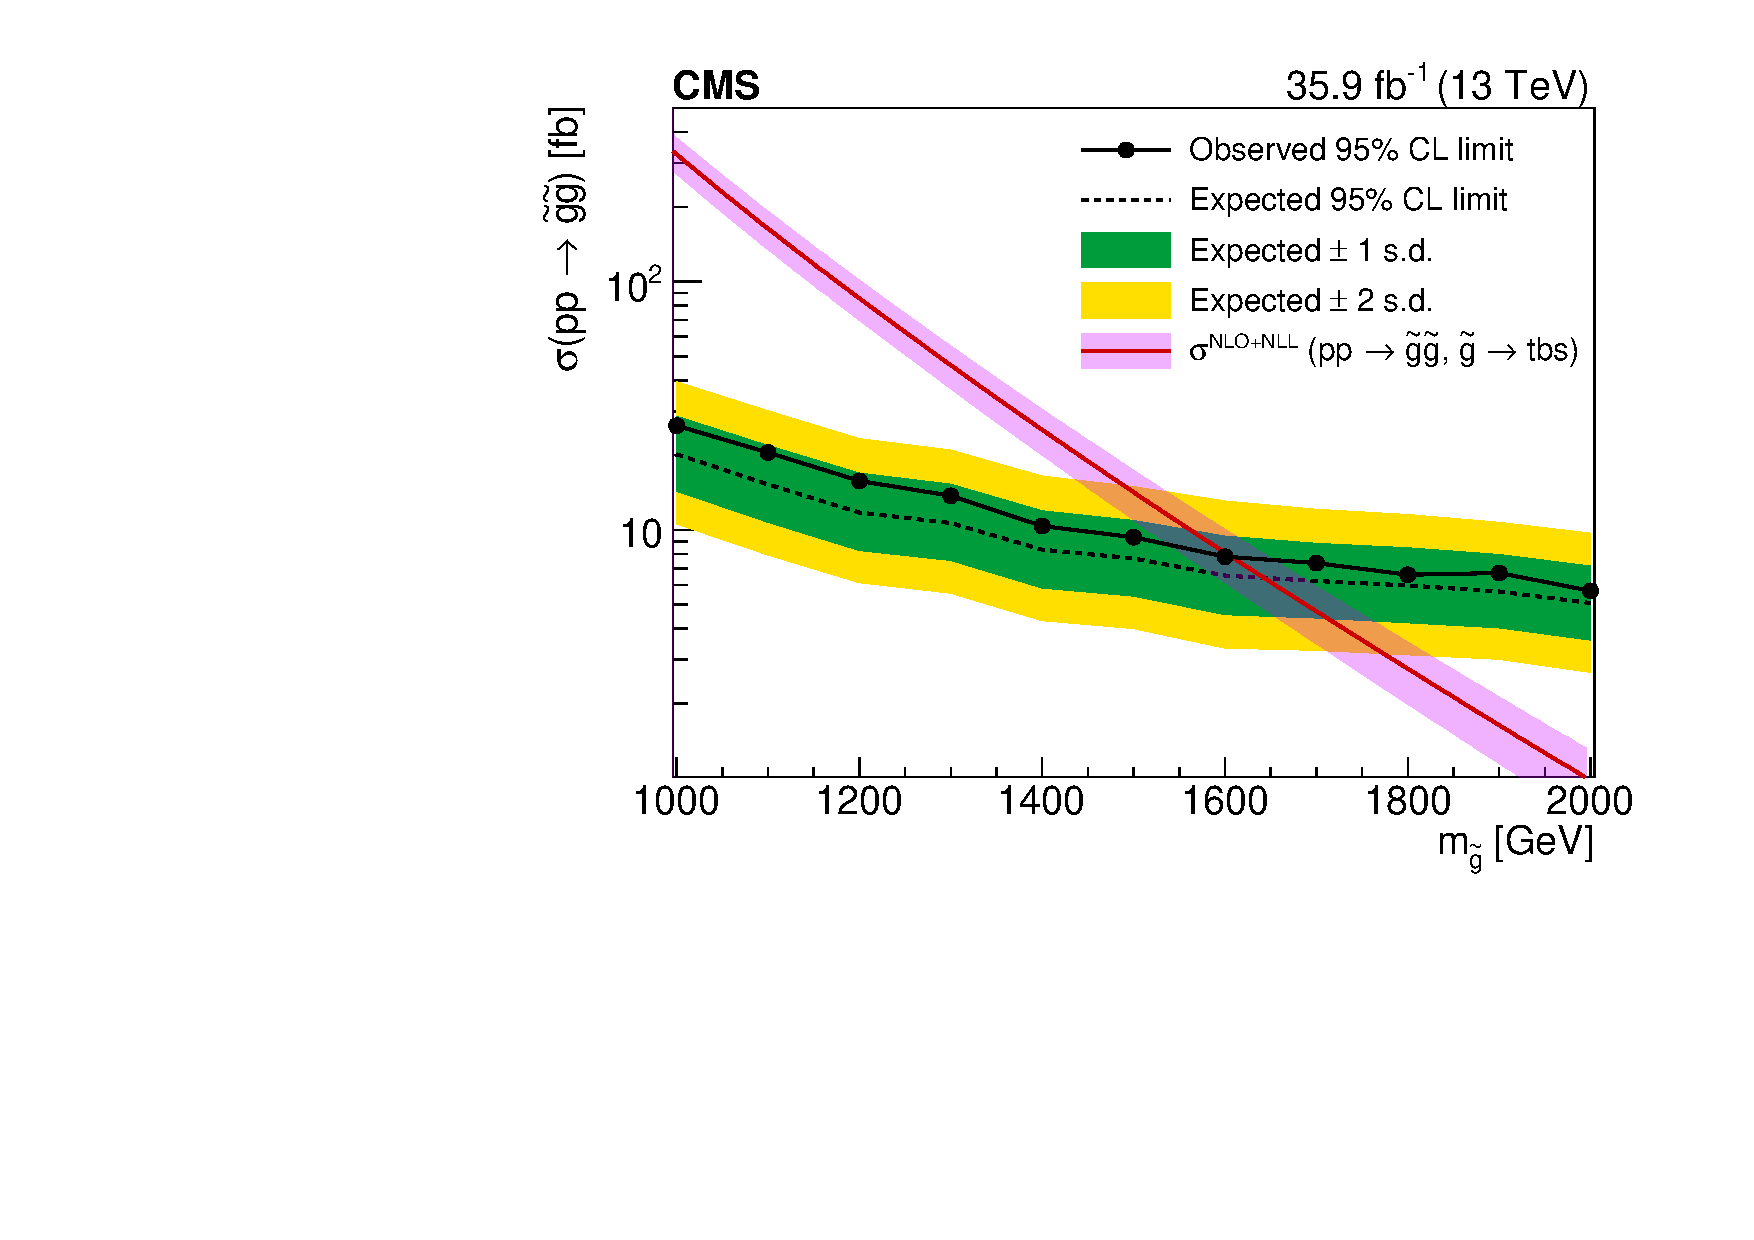
\includegraphics[angle=0,width=0.80\columnwidth]{fig/limits.pdf}
\caption{Cross section upper limits at 95\% CL for a model of gluino pair production with $\glu \to tbs$ compared to the gluino pair production cross section.
The theoretical uncertainties in the cross section are shown as a band around the
red line~\cite{XSecgluinogluino}.
The expected limits (dashed line) and their $\pm1$~s.d.\ and $\pm2$~s.d.\ variations are shown as green and yellow bands, respectively.
The observed limit is shown by the solid line with dots.}
\label{fig:limits}
\end{figure}

\end{section}
